\documentclass[smallextended]{svjour3}
\usepackage{fix-cm}
\usepackage[T1]{fontenc}
\usepackage[utf8]{inputenc}
\usepackage{mathptmx}
\usepackage{amsmath,amssymb,graphicx,booktabs,tabularx,url}
\usepackage{placeins}
\usepackage[numbers,sort&compress]{natbib}
\usepackage[hidelinks]{hyperref}
\journalname{Computing}
\smartqed
\setlength{\emergencystretch}{2em}
\newcommand{\CollegePRDelta}{-0.90780}
\newcommand{\CollegePRLoss}{9.01}
\newcommand{\CollegePRSaving}{86.44}
\newcommand{\CollegePRfiveDelta}{-0.43094}
\newcommand{\CollegePRfiveLoss}{4.28}
\newcommand{\CollegePRfiveSaving}{82.83}
\newcommand{\CollegeDegreeDelta}{0.00000}
\newcommand{\CollegeDegreeLoss}{0.00}
\newcommand{\CollegeDegreeSaving}{86.59}
\newcommand{\GrqcPRDelta}{-0.25082}
\newcommand{\GrqcPRLoss}{5.07}
\newcommand{\GrqcPRSaving}{92.70}
\newcommand{\GrqcPRfiveDelta}{0.00000}
\newcommand{\GrqcPRfiveLoss}{0.00}
\newcommand{\GrqcPRfiveSaving}{88.14}
\newcommand{\GrqcDegreeDelta}{0.00000}
\newcommand{\GrqcDegreeLoss}{0.00}
\newcommand{\GrqcDegreeSaving}{92.77}
\newcommand{\WikiPRDelta}{-40.69334}
\newcommand{\WikiPRLoss}{73.01}
\newcommand{\WikiPRSaving}{96.42}
\newcommand{\WikiPRfiveDelta}{-13.53012}
\newcommand{\WikiPRfiveLoss}{24.28}
\newcommand{\WikiPRfiveSaving}{91.98}
\newcommand{\WikiDegreeDelta}{0.00000}
\newcommand{\WikiDegreeLoss}{0.00}
\newcommand{\WikiDegreeSaving}{96.26}

\begin{document}
\title{Evaluating Candidate-Restricted Influence Maximization: Effects of Selection Budget and Ranking Precision}
\titlerunning{Evaluating candidate-restricted influence maximization}
\author{\mbox{Jiayue Sun} \and \mbox{Binbin Yong} \and \mbox{Junjie An} \and \mbox{Tianyu Bo} \and \mbox{Shuai Li}}
\authorrunning{Jiayue Sun et al.}
\institute{Jiayue Sun \at School of Artificial Intelligence, Lanzhou University, Lanzhou 730000, China
\and Binbin Yong (corresponding author) \at School of Information Science and Engineering, Lanzhou University, Lanzhou 730000, China \\
\email{yongbb14@lzu.edu.cn}
\and Junjie An, Tianyu Bo and Shuai Li \at Lanzhou University, Lanzhou, China}
\date{}
\maketitle
\begin{abstract}
Candidate restriction speeds up greedy influence maximization by letting the search consider only a small set of top-ranked vertices. Its quality is usually judged against full-candidate greedy selection, yet that reference is itself optimized on a finite sample of diffusion worlds, and the restricted pool depends on how precisely the ranking is computed. We examine how these two factors, the selection budget and the ranking precision, shape the comparison. Full and restricted greedy selection share the graph, the selection worlds and the tie rule, and every selected seed set is evaluated on 10,000 independent worlds. On three SNAP networks under the independent-cascade model, PageRank-4k exceeds the full reference on ca-GrQc by a mean 5.6\% of incremental spread at 80 selection worlds but falls 5.1\% below it at 1,280. In a post-hoc analysis, tightening the PageRank tolerance from $10^{-6}$ to $10^{-12}$ exchanges two of the 20 candidates, after which mean spread for the restricted method exceeds the reference at all three budgets. On four contact graphs, 16 of 40 reference sets change between 1,280 and 5,120 worlds, while mean spread rises by only 0.011 nodes. At 1,280 worlds, a 20-vertex degree pool reproduces all 15 reference seed sequences and reduces selection time by more than 98\% relative to exhaustive search, whereas 20-vertex PageRank pools lose 5--73\% of incremental spread. Evaluations of candidate restriction should therefore report the admitted candidates and measure the spread of the selected seeds on independent worlds.
\keywords{influence maximization \and Monte Carlo simulation \and candidate restriction \and evaluation methodology \and reproducibility}
\end{abstract}

\section{Introduction}
Influence maximization asks for a set of $k$ seed vertices that maximizes expected spread under a given diffusion model \cite{ref1}, a formulation of targeted seeding problems such as choosing initial adopters in a social network. The greedy algorithm repeatedly adds the vertex with the largest estimated marginal gain, and because each estimate requires Monte Carlo simulation, its cost grows with both the number of vertices and the number of sampled diffusion worlds. Lazy evaluation, reuse of sampled realizations and sampling-based solvers reduce this cost in different ways \cite{ref7,ref8,ref2}. Candidate restriction takes a simpler route: it ranks vertices by an inexpensive score, such as degree or PageRank, and lets greedy search consider only the top $q$. Whether this pays off depends on how much spread the restricted search retains for the computation it saves.

That trade-off is usually measured against full-candidate greedy selection, which is treated as a fixed benchmark. The benchmark, however, is itself the output of a sampled computation. Both the full and the restricted search optimize an objective estimated from $W$ sampled worlds, so increasing $W$ can change the seeds chosen by either search, and the gap between them reflects changes on both sides. The candidate pool introduces a second, earlier source of variation. PageRank is computed iteratively to a finite tolerance, and when scores near the cutoff are close, a small numerical change can exchange vertices at the pool boundary. Seed-set agreement cannot separate these effects, because two different seed sets may reach almost the same number of vertices.

We therefore compare full and restricted greedy selection in a paired design (Fig.~\ref{fig:evaluation-mechanism}). Both searches use the same graph, the same nested prefix of selection worlds and the same tie rule; only the set of eligible vertices differs. Every selected seed set is then evaluated on a separate family of 10,000 worlds, so that each comparison becomes a paired spread difference measured in nodes. The design addresses three questions: whether ranking tolerance can change the outcome of a budget comparison, how much spread changes when the selected seeds change, and how much selection time each restriction saves at a given loss.

The main experiments use three SNAP networks, CollegeMsg (communication), ca-GrQc (collaboration) and wiki-Vote (voting), chosen before any seed sets or spreads were inspected. An earlier stage of this project examined four small contact graphs; we use those results as a point of comparison and test whether they carry over to the larger networks. The ranking-tolerance comparison was added after the main results were available and is reported as a post-hoc analysis.

The main contributions are:
\begin{enumerate}
\item[(1)] \textbf{We show that ranking precision can reverse the outcome of a budget comparison.} On ca-GrQc, PageRank-4k at the default tolerance exceeds the full reference at $W=80$ but falls below it at $W=320$ and 1,280. Tightening the tolerance exchanges two of the 20 candidates, after which the mean gap is positive at all three budgets (Table~\ref{tab:precision-output}).
\item[(2)] \textbf{We separate changes in the selected set from changes in spread.} Paired evaluation on independent worlds shows that, on the contact graphs, 16 of 40 reference sets change between $W=1280$ and 5,120 while mean spread rises by only 0.011 nodes, with individual differences of both signs.
\item[(3)] \textbf{We quantify the quality--cost trade-off of candidate restriction.} At $W=1280$, Degree-4k reproduces all 15 reference seed sequences on the SNAP networks while reducing selection time by 98.4--99.7\% relative to exhaustive full-candidate search. PageRank-4k reproduces none, and enlarging its pool to 5\% of the vertices narrows, but does not close, the loss on the two directed networks.
\end{enumerate}

\begin{figure}[t]
\centering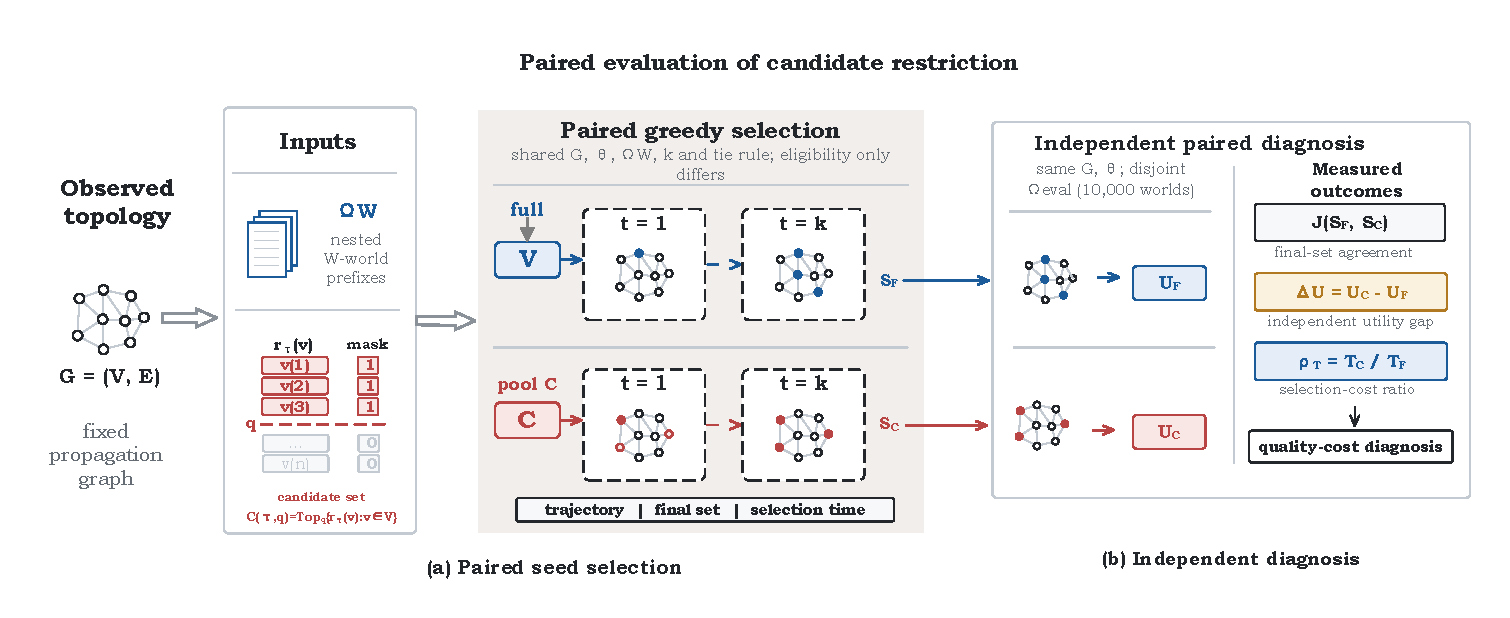
\includegraphics[width=\linewidth]{FigEvaluationMechanism.pdf}
\caption{Paired evaluation design. (a) Full and restricted greedy selection share the graph, the propagation parameters $\theta$, the nested prefix of $W$ selection worlds, the seed budget $k$ and the tie rule. They differ only in the eligible set: the restricted method searches the pool $C(\tau,q)$ of the $q$ top-ranked vertices, with scores computed at tolerance $\tau$. (b) Both selected sets are evaluated on a shared family of $M=10{,}000$ worlds, disjoint from the selection worlds. The outputs are the spread difference $\Delta U$ (restricted minus full), the final-set Jaccard similarity $J$ and the selection-time ratio $\rho_T$.}\label{fig:evaluation-mechanism}
\end{figure}

\section{Related work}
\paragraph{Efficient greedy selection.} Kempe et al. show that expected spread under the independent-cascade model is monotone and submodular, which gives greedy selection its approximation guarantee \cite{ref1}. CELF uses submodularity to skip re-evaluations of marginal gains that cannot change the current choice \cite{ref7}. StaticGreedy fixes one set of sampled realizations for the whole search, so that every candidate is scored on the same coverage objective \cite{ref8}, and IMM replaces forward simulation with a sampling-based solver that carries approximation guarantees \cite{ref2}. These methods make a given objective cheaper to optimize. Candidate restriction instead shrinks the feasible set, and its effect on spread depends on which vertices a particular truncated ranking leaves out. In our experiments the simulator and the greedy rule stay fixed, and only the eligible set, the selection budget or the ranking tolerance changes.

\paragraph{Influence estimation and seed search.} Rui et al. estimate influence from multiple neighbourhood levels \cite{ref12}, Fan et al. search for seeds with a discrete Harris hawks optimizer \cite{ref13}, and Ko et al.'s MONSTOR+ predicts spread on unseen graphs \cite{ref19}. Each of these methods supplies its own estimator or search procedure. We study a narrower role for a ranking: it decides only which vertices greedy search may select, while propagation and evaluation still run on the complete graph. In this role, the quality of a ranking appears as candidate coverage, that is, whether its pool contains the vertices that the full search would choose.

\paragraph{Evaluation of influence-maximization methods.} Li et al. survey the field \cite{ref9}, and Arora et al. benchmark the spread and running time of established methods \cite{ref16}. Yanchenko et al. review formulations on temporal networks \cite{ref11}, and Aral and Dhillon study influence maximization under empirically estimated influence models \cite{ref15}. Together, these studies tie any comparison of algorithms to a diffusion model, a network representation and an evaluation protocol. Our study concerns the protocol. When a cheaper search is compared with a sampled full-candidate reference, we ask how much of the observed gap comes from the restriction itself and how much from the selection budget and the ranking computation, and we measure each contribution on independent evaluation worlds.

\section{Methods}
We compare full and restricted greedy selection on the same propagation graph. Section~\ref{sec:paired} defines the selection objective and the terms used throughout, Section~\ref{sec:coupling} the construction of selection and evaluation worlds, and Section~\ref{sec:cost} the cost measurement. Network statistics and parameter values are given in Section~\ref{sec:experimental-setup}.
\subsection{Paired greedy selection}\label{sec:paired}
Let $G=(V,E)$ be a directed propagation graph and $S$ a seed set of size $k$. Under the independent-cascade model, each newly activated vertex gets one opportunity to activate each inactive outgoing neighbour with probability $p$. Propagation stops after $h$ rounds. For a random world $\omega$, let $f_h(S;\omega)$ denote total activated vertices, including seeds. Greedy selection uses the sampled objective
\begin{equation}
\widehat\sigma_W(S)=\frac{1}{W}\sum_{w=1}^{W}f_h(S;\omega_w).
\end{equation}
In each round, greedy selection evaluates every unselected eligible vertex $v$ and adds the one with the largest integer total $W\widehat\sigma_W(S\cup\{v\})$. Comparing integer totals rather than floating-point means makes ties exact, and remaining ties are broken by the lexicographic order of original node IDs. Full selection uses $C=V$ and restricted selection a pool $C\subset V$; in both cases propagation runs on the complete graph.

We use the following terms throughout. A \emph{method} is a rule that defines the eligible set: full selection, or a restricted pool such as Degree-4k or PageRank-5\%. A \emph{replicate} is one computational repetition with its own families of selection and evaluation worlds, identified by a number (1101--1105 on the SNAP networks). A \emph{configuration} fixes the graph, the replicate, the selection budget $W$ and the world coupling; all methods in a configuration share the same worlds, seed budget $k$ and tie rule. The \emph{full reference} is full selection in the same configuration, and every restricted method is compared with it.

In a budget sweep, the full reference and each restricted method are rerun at every $W$ on the same nested prefix of selection worlds, while the candidate pool stays fixed. A change in their gap across $W$ can therefore come from either search. The ranking tolerance $\tau$ and the pool size $q$ are varied separately from $W$.

Degree is the number of distinct out-neighbours. PageRank is computed on the unweighted directed graph with the NetworkX 3.5 defaults: damping 0.85, uniform personalization and dangling-node handling, tolerance $\tau=10^{-6}$ and at most 100 iterations \cite{networkxpr}. Iteration stops when the $L_1$ change between successive score vectors falls below $n\tau$, where $n=|V|$. Vertices are sorted by decreasing score, with ties broken lexicographically. A pool contains the top $q=\min(n,4k)$ vertices (4k pools) or the top $q=\lceil 0.05n\rceil$ vertices (5\% pools). Event-weighted degree counts messages sent on CollegeMsg and retained contact records incident to each vertex on the undirected contact networks. Each contact is represented by reciprocal arcs, giving each endpoint one outgoing record per retained contact (Weighted-4k and Weighted-5\%). As a baseline, three random pools of size $4k$ are drawn for each graph and replicate and held fixed across budgets and couplings.

\subsection{World coupling and independent evaluation}\label{sec:coupling}
The primary experiments use \emph{step coupling}, in which each random draw is indexed by world, propagation step, source and target. For any fixed seed set, this coupling reproduces the independent-cascade distribution of spread. The sampled objective, however, need not be monotone: seeding an intermediate vertex moves its activation attempts to an earlier step and hence to different draws, which can lower the realized spread (Online Resource 1 gives a counterexample). We retain the step coupling used in the earlier experiments for comparability and use fixed-edge sampling as a control. \emph{Fixed-edge coupling} draws each edge once per world. Its sampled objective counts the vertices reachable from $S$ within $h$ live edges and is monotone and submodular. At every round under both couplings, greedy search enumerates every eligible vertex that has not yet been selected. We use the same exhaustive search in both couplings. CELF can reuse marginal gains as upper bounds for the fixed-edge coverage objective; using that shortcut for the step-coupled objective would require a diminishing-returns guarantee. Each restricted method is compared with the full reference under its own coupling.

Selection worlds form nested prefixes: raising $W$ appends worlds without redrawing the earlier ones. Evaluation uses $M=10{,}000$ worlds per graph, replicate and coupling. These worlds are disjoint from the selection worlds and shared by all methods and budgets, both in the SNAP experiments and in the 520-configuration extension of the contact-graph study. Separate keys distinguish graphs, replicates and random-pool draws.

For restricted seeds $S_C$ and full-reference seeds $S_F$, define the paired evaluation difference on world $i$ as $d_i=f_h(S_C;\eta_i)-f_h(S_F;\eta_i)$. Both sets are selected at the same $W$; positive $d_i$ favors the restricted method. The utility gap in Fig.~\ref{fig:evaluation-mechanism} is
\begin{equation}
\widehat\Delta=\frac{1}{M}\sum_{i=1}^{M}d_i,
\qquad \operatorname{SE}_{\rm MC}=s(d_i)/\sqrt M.
\end{equation}
The interval $\widehat\Delta\pm1.96\operatorname{SE}_{\rm MC}$ measures the Monte Carlo uncertainty of the gap between two fixed seed sets. The standard deviation across replicates reflects how the selected sets themselves vary from one replicate to the next, together with the remaining evaluation noise. For the random pools, the three evaluation vectors are averaged within each replicate before either quantity is computed.

Agreement with the full reference is reported at three levels: an identical ordered seed sequence, an identical final set, and the Jaccard similarity of the final sets. We also record the first round at which the two sequences diverge. Incremental spread is total spread minus the $k$ seeds. The percentage loss of a restricted method is $-100\widehat\Delta/(\widehat\sigma_{\rm full}-k)$, where $\widehat\sigma_{\rm full}$ is the mean total spread of the full reference on the $M$ evaluation worlds of the same replicate; a positive loss means that the restricted set reaches fewer vertices. Losses are computed per replicate and then averaged.

For each graph, we use pre-specified two-sided paired sign tests at $W=1280$, with Holm correction across the three primary comparisons: Degree-4k, PageRank-4k and the mean of the three random pools, each against full selection. The protocol fixed these comparisons before the primary results were inspected. Zero differences are excluded from the tests and reported separately. The analyses of coverage, coupling and budget transitions are descriptive, since replicates measure computational variability on a fixed network.

\subsection{Implementation and cost measurement}\label{sec:cost}
The implementation uses Numba and records, for each configuration and method, the candidate IDs, the selected sequence, the integer totals of every round and the per-world evaluation values. Online Resource 1 describes the reproduction and verification procedures.

Selection time covers greedy search and the lexicographic sorting of candidates; graph preparation, world generation and evaluation are timed separately. To estimate the cost of a complete run in a warm process, we add the separately measured costs of parsing, graph construction and one method's ranking and pool construction (median of five repeats) to the recorded costs of preparing selection worlds, selecting seeds, preparing evaluation worlds and evaluating. This assembled cost excludes imports, just-in-time compilation, downloads and output writing.

Timing variability is assessed with five repeats in randomized method order on replicate 1101 at $W=320$. All cost comparisons are made against this implementation's exhaustive full-candidate search and use the default PageRank tolerance; the tighter tolerance enters only the quality analysis.

\paragraph{Use of AI tools.} OpenAI Codex assisted with basic code development and manuscript drafting. The authors take responsibility for the final manuscript.

\section{Experimental setup}\label{sec:experimental-setup}
We study three SNAP networks under simulated independent-cascade diffusion with $k=5$, $p=0.01$ and $h=3$, and use an earlier contact-graph study from this project as a point of comparison.

\paragraph{Inputs and outputs.} Each run takes a processed graph with its arc directions, the diffusion parameters $k$, $p$ and $h$, a selection budget $W$ and a candidate rule. The ranking tolerance $\tau$ and the cutoff $q$ determine the restricted pool, while the propagation graph stays intact. Selection returns an ordered sequence of $k$ seeds and its selection time. Evaluation takes the final set and the $M$ evaluation worlds of the replicate, and returns total spread, incremental spread and the paired difference from the full reference at the same $W$. Tables~\ref{tab:primary} and~\ref{tab:case} show these outputs together with candidate counts and original node IDs.

\subsection{Networks and preprocessing}
We selected three SNAP networks of different types before inspecting any seed sets or spreads \cite{snap}: CollegeMsg (communication), ca-GrQc (collaboration) and wiki-Vote (voting). Table~\ref{tab:data} lists their processed sizes and candidate coverage; all weak components are retained.
\begin{table}[htbp]
\caption{Processed SNAP networks. Arcs are directed propagation arcs. The 4k fraction is the share of vertices in a 20-vertex pool; the 5\% pool contains $\lceil 0.05n\rceil$ vertices.}\label{tab:data}
\begin{tabular}{lrrrr}
\toprule
Graph & Nodes & Arcs & 4k fraction & 5\% pool \\
\midrule
CollegeMsg & 1,438 & 13,397 & 1.391\% & 72 \\
ca-GrQc & 5,241 & 28,968 & 0.382\% & 263 \\
wiki-Vote & 7,115 & 103,689 & 0.281\% & 356 \\
\bottomrule
\end{tabular}
\end{table}

CollegeMsg records timestamped messages from sender to receiver \cite{college}. Following the history-window convention of the contact-graph study, we retain the earliest 65\% of distinct timestamps, $\lfloor 0.65\times58{,}911\rfloor=38{,}292$ of 58,911, which covers events up to Unix time 1085640224. After removing self-messages, we use the 38,939 retained events both to construct the directed graph and to rank vertices by outgoing message count. Repeated messages between the same pair form a single propagation arc but each count toward the sender's message count, and propagation uses the uniform $p$ regardless of message count.

ca-GrQc connects coauthors \cite{grqc}. We remove self-loops, merge duplicate pairs and add arcs in both directions. Vertex 12295 appears only in a self-loop and is dropped, which leaves 5,241 vertices instead of the 5,242 listed by SNAP. In wiki-Vote, arcs point from voter to votee \cite{signed,links}; we remove self-loops and duplicate arcs and keep the original direction, so that influence is simulated as flowing from voters to the users they vote for. Because the two static datasets carry no event counts, event-weighted pools are used only on CollegeMsg. The processed graphs have 2 (CollegeMsg), 354 (ca-GrQc) and 24 (wiki-Vote) weak components. Original IDs are stored as strings and sorted lexicographically to index vertices and to break ties in ranking and in greedy selection. Hashes of the raw and processed files are listed in the data manifest.

The earlier stage of this project used four contact graphs with 75--402 vertices, derived from workplace, conference and rural Kenya data \cite{ref3,ref4,ref5,ref6}. It began with 42 configurations and was later extended to 520 configurations with ten replicates per graph. The extension adds a budget scan up to $W=5120$, four local changes to $(p,h)$, fixed-edge sampling, a larger seed budget of $k=20$, and two fixed 2,000-node synthetic graphs \cite{ref17,ref18}; the parameter variations reuse the configurations of the default budget scan. Online Resource 1 reports the contact-graph results in full.

\subsection{Primary design and ranking-precision analysis}
Table~\ref{tab:settings} summarizes the design on the SNAP networks. The primary experiments cross three graphs, five replicates and three selection budgets, $W\in\{80,320,1280\}$, which gives 45 configurations under step coupling. Nine further configurations use fixed-edge coupling at $W=320$ on replicates 1101--1103. Every configuration runs full selection, Degree-4k, PageRank-4k, Degree-5\%, PageRank-5\% and three random 4k pools, and CollegeMsg adds Weighted-4k and Weighted-5\%. Over the 18 configurations per graph, this amounts to $18\times(10+8+8)=468$ method runs.

\begin{table}[htbp]
\caption{Experiment settings on the SNAP networks.}\label{tab:settings}
\begin{tabularx}{\linewidth}{lX}
\toprule
Quantity & Setting \\
\midrule
Diffusion & Independent cascade; uniform $p=0.01$; horizon $h=3$; $k=5$ seeds \\
Primary selection & Step coupling; $W\in\{80,320,1280\}$; replicates 1101--1105 \\
Evaluation & $M=10{,}000$ worlds per graph, replicate and coupling, shared across methods and budgets \\
Pool sizes & $4k=20$ or $\lceil0.05n\rceil$; three random pools of size 20 per replicate \\
Fixed-edge control & $W=320$; replicates 1101--1103 \\
Default PageRank & Damping 0.85; $\tau=10^{-6}$; at most 100 iterations \\
Strict PageRank (post-hoc) & $\tau=10^{-12}$; at most 1,000 iterations; pool unchanged at $10^{-14}$ \\
Repeated timing & Five repeats per method in randomized order; replicate 1101, $W=320$ \\
\bottomrule
\end{tabularx}
\end{table}

The ranking-precision analysis was added after the primary results were available. On the original five replicates, it recomputes PageRank with $\tau=10^{-12}$ and at most 1,000 iterations, reruns the restricted search at each $W$, and compares the result with the original full reference on the same evaluation worlds. Recomputing at $\tau=10^{-14}$ leaves the pool membership unchanged. Online Resource 1 describes the two stages of this analysis.

\subsection{Randomization, execution and reproducibility}
All random draws are derived from hash keys that separate graphs, replicates, and the selection and evaluation families. Raising $W$ appends selection worlds without resampling the prefix, and we verify that selection and evaluation identifiers never overlap. Random pools use a separate key and remain fixed across budgets and couplings. Online Resource 1 (``Executable reproduction procedure'') gives the exact keys, the identifier construction and the mapping from hashes to draws.

Experiments run as a single serial worker on Windows with Python 3.13.0, NumPy 2.3.3, NetworkX 3.5, SciPy 1.16.1 and Numba 0.68.0, with BLAS and OpenMP limited to one thread, on a host with 20 physical cores and about 32 GiB of RAM. Just-in-time compilation is warmed up before any timed configuration, and methods run in randomized order to avoid systematic order effects.

\section{Results}
\subsection{Post-hoc sensitivity of the budget comparison to PageRank tolerance}
On ca-GrQc, the direction of the PageRank-4k comparison depends on the tolerance at which PageRank is computed (Fig.~\ref{fig:precision-budget}, Table~\ref{tab:precision-output}). At the default tolerance, PageRank-4k exceeds the full reference by a mean 5.6\% of incremental spread at $W=80$, then falls 2.5\% and 5.1\% below it at $W=320$ and 1,280. At the strict tolerance, it exceeds the reference at all three budgets, by 11.3\%, 3.0\% and 0.5\%. This analysis is post-hoc, and the gaps involved are small: at most 0.49 nodes in magnitude, against a full-reference incremental spread of 4.9 nodes at $W=1280$, with across-replicate standard deviations of 0.08--0.27 nodes.

Two vertices change at the pool boundary. Tightening the tolerance removes vertices 1488 and 19865 from the 20-vertex pool and admits 17655 and 6610, which changes the final seed set on all five replicates at every budget. The selection budget still matters within the strict pool: raising $W$ changes the selected set on three of five replicates from 80 to 320 worlds and on two from 320 to 1,280. At $W=1280$ the strict gap averages $+0.026$ nodes and ranges from $-0.041$ to $+0.179$ across replicates, so it lies on both sides of zero.

On the two directed networks, the PageRank-4k losses persist at the tighter tolerance. On CollegeMsg, the two tolerances yield identical pools, seeds and evaluations, with losses of 9.3\%, 8.5\% and 9.0\% at the three budgets. On wiki-Vote one candidate changes, but the loss at the strict tolerance remains about 74\% at every budget.

\begin{table}[htbp]
\caption{PageRank-4k on ca-GrQc at the default ($\tau=10^{-6}$) and strict ($\tau=10^{-12}$) tolerance. Gaps are restricted minus full-reference spread at the same $W$, in nodes, averaged over five replicates, with the standard deviation across replicates in parentheses. Changed sets counts the replicates on which the two tolerances select different final sets.}\label{tab:precision-output}
\centering\begin{tabular}{rrrr}\toprule
$W$ & Default gap (SD) & Strict gap (SD) & Changed sets \\ \midrule
80 & +0.23606 (0.27402) & +0.48570 (0.24999) & 5/5 \\
320 & -0.12632 (0.18077) & +0.13804 (0.17387) & 5/5 \\
1280 & -0.25082 (0.07636) & +0.02608 (0.09155) & 5/5 \\
\bottomrule\end{tabular}
\end{table}

\begin{figure}[t]
\centering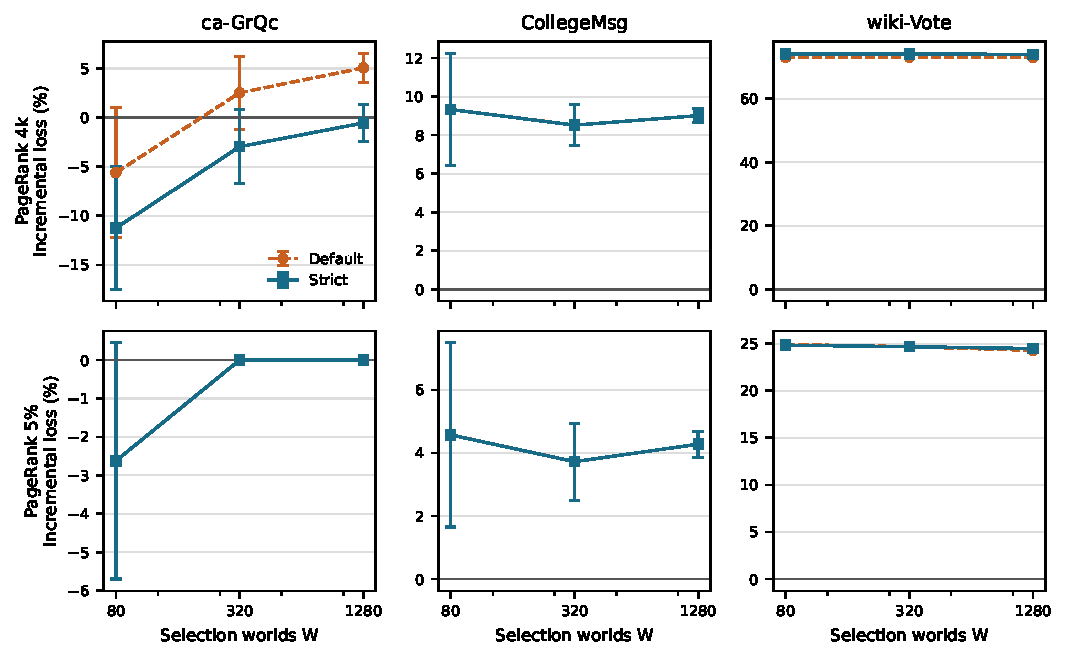
\includegraphics[width=\linewidth]{Fig4.pdf}
\caption{Incremental-spread loss of PageRank pools relative to the full reference at the same $W$, at the default ($\tau=10^{-6}$) and strict ($\tau=10^{-12}$) tolerance. Top row: 4k pools; bottom row: 5\% pools. Points are means over five replicates and bars are standard deviations across replicates; a positive loss means that the restricted set reaches fewer vertices. On ca-GrQc, the default PageRank-4k loss changes sign across budgets, whereas the strict-tolerance loss stays below zero. On CollegeMsg and wiki-Vote, the losses persist at both tolerances.}\label{fig:precision-budget}
\end{figure}

\subsection{A change in the reference set need not change its spread}
The full reference often changes as $W$ grows, but the resulting change in spread is small and can take either sign (Fig.~\ref{fig:transitions}). Between $W=320$ and 1,280, all five ca-GrQc reference sets change, and their spread changes by a mean $+0.127$ nodes, ranging from $-0.027$ to $+0.241$. On CollegeMsg one set changes, which raises the five-replicate mean spread by 0.053 nodes. On wiki-Vote some selection orders change but no final set does; because spread depends only on the set, every paired difference is exactly zero. Of the six changed sets, four have 95\% Monte Carlo intervals above zero, and the intervals of the other two, both on ca-GrQc, include zero.

The contact-graph study shows the same pattern at larger budgets. Under step coupling, 16 of 40 reference sets change between $W=1280$ and 5,120, while spread changes by a mean $+0.011$ nodes (range $-0.038$ to $+0.118$). Under fixed-edge coupling, 29 of 40 sets change between $W=320$ and 1,280, with a mean change of $+0.062$ nodes (range $-0.011$ to $+0.257$). Each transition is evaluated on a shared family of worlds within its own coupling, and the two span different budget ranges.
\begin{figure}[t]
\centering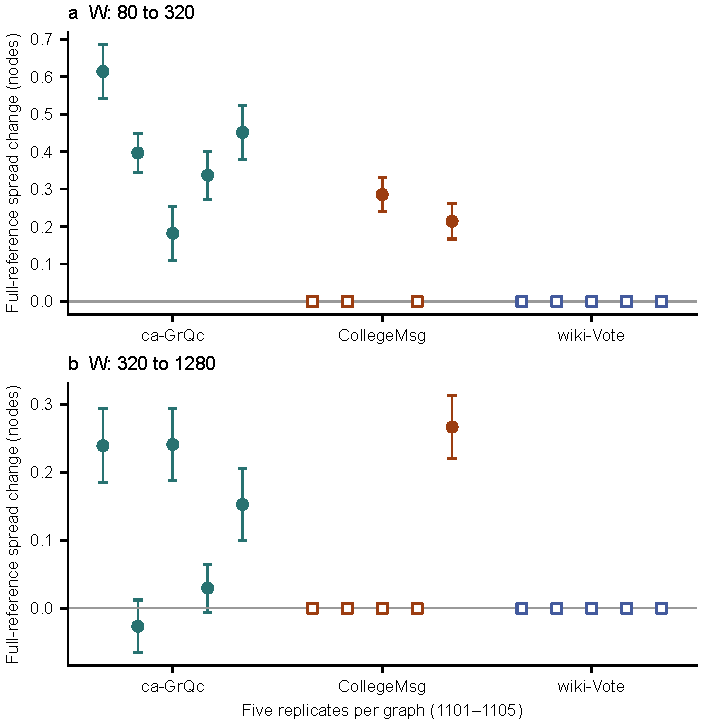
\includegraphics[width=\linewidth]{Fig2.pdf}
\caption{Change in full-reference spread between two selection budgets (higher minus lower $W$) for each replicate on the SNAP networks: (a) $W=80$ to 320; (b) $W=320$ to 1,280. Replicates 1101--1105 run from left to right within each graph. Filled circles mark replicates whose final set changed, and hollow squares mark unchanged sets. Bars are unadjusted 95\% Monte Carlo intervals from 10,000 paired evaluation worlds. Vertical scales differ between panels.}\label{fig:transitions}
\end{figure}

\subsection{Degree pools reproduce the reference, PageRank pools do not}
At $W=1280$, Degree-4k reproduces every full-reference seed sequence on all three SNAP networks while searching only 20 candidates (Table~\ref{tab:primary}). Default PageRank-4k reproduces none and loses a mean \GrqcPRLoss{}\%, \CollegePRLoss{}\% and \WikiPRLoss{}\% of incremental spread on ca-GrQc, CollegeMsg and wiki-Vote. The contact-graph study found near-complete agreement for both rankings: PageRank-4k reproduced 40 of 40 sequences at $W=5120$ and Degree-4k 39 of 40. The earlier PageRank agreement thus varies across the networks and budgets examined here.

\begin{table}[htbp]
\caption{Results on the SNAP networks at $W=1280$, averaged over five replicates. PR denotes PageRank at the default tolerance. Incremental spread excludes the $k=5$ seeds; the gap is restricted minus full-reference spread, in nodes; agreement counts replicates with an identical ordered seed sequence.}\label{tab:primary}
\centering\begin{tabular}{lrrrr}\toprule
Graph / method & Candidates & Incremental & Gap & Agreement \\ \midrule
\multicolumn{5}{l}{\textit{ca-GrQc}} \\
Full & 5241 & 4.934 & --- & --- \\
Degree-4k & 20 & 4.934 & +0.00000 & 5/5 \\
PR-4k & 20 & 4.683 & -0.25082 & 0/5 \\
PR-5\% & 263 & 4.934 & +0.00000 & 5/5 \\
\addlinespace
\multicolumn{5}{l}{\textit{CollegeMsg}} \\
Full & 1438 & 10.072 & --- & --- \\
Degree-4k & 20 & 10.072 & +0.00000 & 5/5 \\
PR-4k & 20 & 9.164 & -0.90780 & 0/5 \\
PR-5\% & 72 & 9.641 & -0.43094 & 0/5 \\
\addlinespace
\multicolumn{5}{l}{\textit{wiki-Vote}} \\
Full & 7115 & 55.736 & --- & --- \\
Degree-4k & 20 & 55.736 & +0.00000 & 5/5 \\
PR-4k & 20 & 15.043 & -40.69334 & 0/5 \\
PR-5\% & 356 & 42.206 & -13.53012 & 0/5 \\
\bottomrule\end{tabular}
\end{table}

In the pre-specified tests at $W=1280$, the PageRank-4k difference and the random-pool mean difference from full selection are negative on every replicate of every graph, which gives an unadjusted sign-test $p=0.0625$ and a Holm-adjusted $p=0.1875$. With five replicates, 0.0625 is the smallest attainable two-sided $p$-value, so these consistent losses cannot reach conventional significance. The Degree-4k differences are exactly zero. Online Resource 1 reports the paired effect sizes and the complete test results.

Table~\ref{tab:case} illustrates the contrast on wiki-Vote replicate 1101. The 20-vertex degree pool returns the same five seeds, in the same order, as the full search over 7,115 vertices, and reaches a mean total spread of 60.8 nodes. Default PageRank-4k selects five different seeds and reaches 19.9 nodes; enlarging its pool to 356 vertices raises this to 47.2 nodes.

\begin{table}[htbp]
\caption{Selected seeds on wiki-Vote, replicate 1101 ($k=5$, $p=0.01$, $h=3$, $W=1280$, $M=10{,}000$, step coupling; 7,115 vertices and 103,689 arcs). PR uses the default tolerance. Arrows give the selection order; total spread includes the seeds and is estimated on the evaluation worlds.}\label{tab:case}
\begin{tabularx}{\linewidth}{lXr}\toprule
Method & Selected seed sequence & Total spread \\ \midrule
Full & $2565\to 766\to 11\to 457\to 2688$ & 60.8455 \\
Degree-4k & $2565\to 766\to 11\to 457\to 2688$ & 60.8455 \\
PR-4k & $3352\to 2237\to 2328\to 2654\to 1297$ & 19.9366 \\
PR-5\% & $2565\to 1166\to 1549\to 1374\to 5524$ & 47.2095 \\
\bottomrule\end{tabularx}
\end{table}

Larger pools reduce the PageRank loss, but by different amounts on different networks. With the 5\% pool, PageRank reproduces all five ca-GrQc references at $W=1280$ and cuts the CollegeMsg loss from \CollegePRLoss{}\% to \CollegePRfiveLoss{}\%. On wiki-Vote the loss falls from \WikiPRLoss{}\% to \WikiPRfiveLoss{}\%, which is still more than a fifth of the reference's incremental spread. On CollegeMsg, event-weighted pools move from a mean gap of $-0.25$ nodes at 4k to exact reproduction of the reference at 5\%.

On wiki-Vote, the two 20-vertex pools draw on different kinds of vertices. The PageRank top 20 have a mean in-degree of 250 and a mean out-degree of 56, whereas the degree top 20 have 70 and 489. The PageRank-4k pool contains none of the five full-reference seeds on any replicate at $W=1280$, and the 5\% pool contains only one. Online Resource 1 gives the seed-level illustration and the complete coverage comparisons.

\subsection{Degree-4k preserves the reference at a fraction of the selection cost}
At $W=1280$, Degree-4k reduces selection time by 98.4--99.7\% relative to exhaustive full-candidate search while reproducing every reference sequence (Table~\ref{tab:cost}). When graph setup, both world families and independent evaluation are included, the saving is \CollegeDegreeSaving{}--\WikiDegreeSaving{}\%, because both methods incur graph and world preparation costs. This estimate includes each method's own ranking or pool-construction cost and its measured evaluation time.

\begin{table}[htbp]
\caption{Selection cost of Degree-4k at $W=1280$, averaged over five replicates. Full and Degree give the measured selection time. The last column gives the saving in an assembled warm-process cost that adds graph setup, preparation of selection and evaluation worlds, and independent evaluation (Section~\ref{sec:cost}).}\label{tab:cost}
\begin{tabular}{lrrrr}
\toprule
Graph & Full (s) & Degree (s) & \shortstack{Selection\\saving (\%)} & \shortstack{Saving including\\evaluation (\%)} \\
\midrule
ca-GrQc & 23.53 & 0.109 & 99.54 & 92.77 \\
CollegeMsg & 5.89 & 0.094 & 98.40 & 86.59 \\
wiki-Vote & 158.94 & 0.520 & 99.67 & 96.26 \\
\bottomrule
\end{tabular}
\end{table}

We also report the fraction of replicates meeting each of six pre-specified loss thresholds (0\%, 1\%, 2.5\%, 5\%, 10\% and 20\%), with loss expressed relative to the full reference's incremental spread within each replicate. At $W=1280$, Degree-4k meets the 0\% threshold on every replicate. Default PageRank-4k meets the 10\% threshold on ca-GrQc and CollegeMsg but misses 20\% on every wiki-Vote replicate, and no random-pool mean meets 20\%. Online Resource 1 lists the fractions for all thresholds and the corresponding costs.

\subsection{Results under fixed-edge coupling and other parameters}
The PageRank losses persist under fixed-edge coupling. At $W=320$, default PageRank-4k trails the fixed-edge full reference by a mean 0.16, 0.93 and 40.6 nodes on ca-GrQc, CollegeMsg and wiki-Vote. Degree-4k reproduces one of the three reference sequences on ca-GrQc and all three on CollegeMsg and wiki-Vote. Online Resource 1 gives the complete control results and the repeated timings.

In the contact-graph study, both rankings reproduce most full-reference sequences in the 160 configurations with non-default parameters at $W=320$: 117 for Degree-4k and 132 for PageRank-4k. Event-weighted pools mostly fall short of full selection, with 117 negative and 43 positive paired differences. Under fixed-edge coupling at $W=1280$, Degree-4k and PageRank-4k reproduce 38 and 40 of 40 reference sequences, whereas Weighted-4k reproduces 5.
\FloatBarrier

\section{Discussion}
\subsection{Why the ca-GrQc comparison changes sign}
The reversal on ca-GrQc comes from the candidate pool, not from the selection budget. At a fixed $W$, the two tolerance settings share the full reference, the sampled objective and the evaluation worlds, and differ only in which vertices are eligible. Exchanging two of the 20 candidates is therefore enough to turn a budget sweep in which the restricted method appears to fall behind the reference into one in which it never does. The budget still has an effect of its own: within the strict pool, raising $W$ changes the selected seeds, and at the highest budget the gap spans zero. A sweep over $W$ thus mixes two processes, the convergence of each search and the composition of the pool, and when the gaps amount to a fraction of a node, the second can decide the outcome.

StaticGreedy controls sampling variation by fixing the sampled realizations throughout the search \cite{ref8}, and our paired design applies the same control to both searches. Ranking and truncation, however, act before the search begins and lie outside this control. Reporting which candidate IDs enter or leave the pool when the tolerance is tightened identifies the changes in eligibility.

\subsection{Seed sequences and seed sets}
Agreement statistics based on seed sequences can overstate how much a change matters. Greedy search produces an ordered sequence, but the diffusion model takes only the final set as input, so on wiki-Vote a reordered sequence left every evaluation count unchanged. When the membership does change, its effect on spread has to be measured: on ca-GrQc, the higher-budget reference sets reached more vertices on some replicates and fewer on others. For seeding decisions the relevant quantity is the paired spread difference, and set agreement serves mainly to diagnose where that difference comes from.

\subsection{Candidate coverage and the cost of exclusion}
Increasing the PageRank pool size recovers part of the spread lost on wiki-Vote. On wiki-Vote, the 20-vertex PageRank pool excluded all five reference seeds, and the 356-vertex pool admitted only one. The larger pool nonetheless raised the five-replicate mean total spread from 20.0 to 47.2 nodes, against 60.7 for the full reference. Thus, at least four of the five seeds in each expanded-pool result differ from the corresponding reference seeds.

The two 20-vertex pools favour opposite directions of the graph. PageRank promotes vertices that receive many votes, whereas degree promotes vertices that cast many. Diffusion follows voter-to-votee arcs, so a vertex with more distinct out-neighbours has more opportunities for first-round activation. This directional difference is consistent with the observed spread gap. Reversing the propagation direction on the same topology would test this interpretation directly.

Benchmarks such as that of Arora et al. report spread and running time side by side \cite{ref16}. Our results add that the same computational budget can buy very different quality depending on which ranking defines the pool. Degree-4k removes most candidate evaluations while reproducing the reference on all 15 graph--replicate pairs at $W=1280$, whereas a PageRank pool of the same size on wiki-Vote loses nearly three quarters of the incremental spread.

\subsection{Scope and limitations}
Our conclusions apply to three SNAP networks with at most 7,115 vertices, under simulated independent-cascade diffusion with $k=5$, $p=0.01$, $h=3$ and $W\le1280$. The diffusion is simulated on observed topologies, so the results describe the behaviour of the algorithms rather than realized social influence. The three-round horizon limits propagation to vertices within three directed steps of a seed. How the degree ranking performs under stronger or longer-range diffusion remains open. The contact-graph study covers other probabilities, horizons and seed budgets, but its pools often contain a large share of the vertices (at $k=20$, every vertex of the Kenya graph and 80 of 91 in invs2013), so agreement there carries less information than agreement with a 20-vertex pool on wiki-Vote.

Replicates measure computational variability on a fixed network, not variation across networks, and with five replicates the sign test cannot fall below $p=0.0625$. The ranking-precision analysis is post-hoc and uses the five original replicates under step coupling; repeating it under fixed-edge coupling would show whether the ca-GrQc result persists under a different world construction. All cost comparisons are made against exhaustive full-candidate search, and the assembled costs are built from separately measured components rather than timed end to end. The relative time saving under a lazy or sampling-based solver requires a separate timing comparison. Finally, the six loss thresholds serve as descriptive comparison points; what loss is acceptable depends on the application.

\section{Conclusion}
Comparisons of candidate-restricted influence maximization depend on two computations that are easy to overlook: the sampled optimization that produces the full reference, and the numerical ranking that defines the pool. On ca-GrQc, exchanging two vertices at the PageRank cutoff was enough to remove an apparent reversal across selection budgets. In the SNAP and contact-graph budget comparisons, changes in seed membership were accompanied by both positive and negative differences in independently estimated spread. On all three SNAP networks, a 20-vertex degree pool reproduced the full reference at a small fraction of its selection cost, whereas PageRank pools of the same size lost spread. We therefore recommend that evaluations of candidate restriction report the candidates near the cutoff and their stability under a tighter ranking tolerance, and measure the spread of the selected seeds on independent worlds. Extending the comparison to larger networks, stronger diffusion and faster reference solvers is the natural next step.

\paragraph{Supplementary information.} Online Resource 1 contains the full result matrix for the SNAP networks, the precision and direction diagnostics, the loss--cost curves, the contact-graph coverage, parameter, coupling and secondary-control tables, and the reproducibility details.
\section*{Statements and Declarations}
\paragraph{Funding.} This work was supported by a provincial undergraduate innovation and entrepreneurship training project.
\paragraph{Competing interests.} The authors declare that they have no competing interests.
\paragraph{Author contributions.} Jiayue Sun: conceptualization, methodology, software, validation, formal analysis, investigation, data curation, visualization, and writing---original draft. Binbin Yong: supervision, methodology, project administration, and writing---review and editing. Junjie An: software, data curation, and writing---review and editing. Tianyu Bo: validation, visualization, and writing---review and editing. Shuai Li: formal analysis, validation, and writing---review and editing. All authors read and approved the final manuscript and agreed to its submission to \textit{Computing}.
\paragraph{Data availability.} The third-party datasets are available from the cited providers under their access terms and are not redistributed. Source records, expected SHA-256 hashes and preprocessing instructions accompany the submission.
\paragraph{Code availability.} Archived source snapshots, configurations, validators, analysis scripts, configuration-level outputs and figure-source tables are supplied with the submission for editorial and peer-review access.
\begin{thebibliography}{99}
\bibitem{ref1} Kempe D, Kleinberg J, Tardos É (2003) Maximizing the spread of influence through a social network. In: ACM SIGKDD, pp 137--146. \url{https://doi.org/10.1145/956750.956769}

\bibitem{ref7} Leskovec J, Krause A, Guestrin C, Faloutsos C, VanBriesen J, Glance N (2007) Cost-effective outbreak detection in networks. In: KDD, pp 420--429. \url{https://doi.org/10.1145/1281192.1281239}

\bibitem{ref8} Cheng S, Shen H, Huang J, Zhang G, Cheng X (2013) StaticGreedy: solving the scalability-accuracy dilemma in influence maximization. In: CIKM, pp 509--518. \url{https://doi.org/10.1145/2505515.2505541}

\bibitem{ref2} Tang Y, Shi Y, Xiao X (2015) Influence maximization in near-linear time: a martingale approach. In: ACM SIGMOD, pp 1539--1554. \url{https://doi.org/10.1145/2723372.2723734}

\bibitem{ref12} Rui X, Yang X, Fan J, Wang Z (2020) A neighbour scale fixed approach for influence maximization in social networks. Computing 102:427--449. \url{https://doi.org/10.1007/s00607-019-00778-5}

\bibitem{ref13} Fan C, Wang Z, Zhang J, Zhao J, Rui X (2024) Influence maximization in social networks based on discrete harris hawks optimization algorithm. Computing 106:327--351. \url{https://doi.org/10.1007/s00607-023-01207-4}

\bibitem{ref19} Ko J, Kim S, Lee K, et al. (2025) Inductive influence estimation and maximization over unseen social networks under two diffusion models. Data Mining and Knowledge Discovery 39:55. \url{https://doi.org/10.1007/s10618-025-01137-z}

\bibitem{ref9} Li Y, Fan J, Wang Y, Tan K-L (2018) Influence maximization on social graphs: a survey. IEEE Transactions on Knowledge and Data Engineering 30:1852--1872. \url{https://doi.org/10.1109/TKDE.2018.2807843}

\bibitem{ref16} Arora A, Galhotra S, Ranu S (2017) Debunking the myths of influence maximization: an in-depth benchmarking study. In: SIGMOD, pp 651--666. \url{https://doi.org/10.1145/3035918.3035924}

\bibitem{ref11} Yanchenko E, Murata T, Holme P (2024) Influence maximization on temporal networks: a review. Applied Network Science 9:16. \url{https://doi.org/10.1007/s41109-024-00625-3}

\bibitem{ref15} Aral S, Dhillon PS (2018) Social influence maximization under empirical influence models. Nature Human Behaviour 2:375--382. \url{https://doi.org/10.1038/s41562-018-0346-z}

\bibitem{networkxpr} NetworkX developers (2025) PageRank, NetworkX 3.5 documentation. \url{https://networkx.org/documentation/networkx-3.5/reference/algorithms/generated/networkx.algorithms.link_analysis.pagerank_alg.pagerank.html}. Accessed 15 October 2026

\bibitem{snap} Leskovec J, Krevl A (2014) SNAP datasets: Stanford large network dataset collection. \url{https://snap.stanford.edu/data}. Accessed 15 October 2026

\bibitem{college} Panzarasa P, Opsahl T, Carley KM (2009) Patterns and dynamics of users' behavior and interaction: Network analysis of an online community. Journal of the American Society for Information Science and Technology 60:911--932. \url{https://doi.org/10.1002/asi.21015}

\bibitem{grqc} Leskovec J, Kleinberg J, Faloutsos C (2007) Graph evolution: densification and shrinking diameters. ACM Transactions on Knowledge Discovery from Data 1(1):2. \url{https://doi.org/10.1145/1217299.1217301}

\bibitem{signed} Leskovec J, Huttenlocher D, Kleinberg J (2010) Signed networks in social media. In: CHI, pp 1361--1370. \url{https://doi.org/10.1145/1753326.1753532}

\bibitem{links} Leskovec J, Huttenlocher D, Kleinberg J (2010) Predicting positive and negative links in online social networks. In: WWW, pp 641--650. \url{https://doi.org/10.1145/1772690.1772756}

\bibitem{ref3} Génois M, Vestergaard CL, Fournet J, Panisson A, Bonmarin I, Barrat A (2015) Data on face-to-face contacts in an office building suggest a low-cost vaccination strategy based on community linkers. Network Science 3:326--347. \url{https://doi.org/10.1017/nws.2015.10}

\bibitem{ref4} Génois M, Barrat A (2018) Can co-location be used as a proxy for face-to-face contacts? EPJ Data Science 7:11. \url{https://doi.org/10.1140/epjds/s13688-018-0140-1}

\bibitem{ref5} Cattuto C, Van den Broeck W, Barrat A, Colizza V, Pinton J-F, Vespignani A (2010) Dynamics of person-to-person interactions from distributed RFID sensor networks. PLoS ONE 5:e11596. \url{https://doi.org/10.1371/journal.pone.0011596}

\bibitem{ref6} Kiti MC, Tizzoni M, Kinyanjui TM, et al. (2016) Quantifying social contacts in a household setting of rural Kenya using wearable proximity sensors. EPJ Data Science 5:21. \url{https://doi.org/10.1140/epjds/s13688-016-0084-2}

\bibitem{ref17} Barabasi A-L, Albert R (1999) Emergence of scaling in random networks. Science 286:509--512. \url{https://doi.org/10.1126/science.286.5439.509}

\bibitem{ref18} Holland PW, Laskey KB, Leinhardt S (1983) Stochastic blockmodels: first steps. Social Networks 5:109--137. \url{https://doi.org/10.1016/0378-8733(83)90021-7}
\end{thebibliography}

\end{document}
